
% NE PAS TOUCHER
%++++++++++++++++++++++++++++++++++++++++
\documentclass[letterpaper,12pt]{article}
\usepackage{tabularx}
\usepackage{amsmath}
\usepackage{graphicx}
\usepackage[margin=1in,letterpaper]{geometry}
\usepackage{cite}
\usepackage[final]{hyperref}
\usepackage{datatool}
\usepackage{caption}
\usepackage{float}
\usepackage{gensymb}

\hypersetup{
	colorlinks=true,
	linkcolor=blue,
	citecolor=blue,
	filecolor=magenta,
	urlcolor=blue
}
%+++++++++++++++++++++++++++++++++++++++++

%	INCLUDES
\graphicspath{ {./ressources/} }

\begin{document}

\title{Automatique}

\author{Seite Alexander}
\date{\today}
\maketitle
\newline

\tableofcontents

\newpage

\section{Exercice 1 : Système masse-ressort (matlab)}
\begin{figure}[h]
        \begin{centering}
        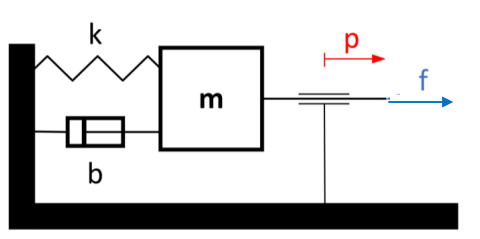
\includegraphics[scale=0.7]{AB.png}
        \end{centering}
\end{figure}

\subsection{A}
\[
	\sum_{}^{}F = ma
\]
\[
	\Leftrightarrow \dot{m} \cdot p(t) = -k\cdot p(t) - b \cdot \dot{p(t)} + f(t)
\]

\subsection{B}
\[
	\mathcal{L} \rightarrow m\cdot s^2 \cdot P(s) = -k \cdot P(s) - b\cdot s \cdot P(s) + F(s)
\]
\[
	\Leftrightarrow G(s) = ...
\]

\subsection{C}

\subsection{D}

\subsection{E}

\subsection{F}


\newpage

\section{Exercice 2 : Système masse-ressort (simulink)}
\begin{figure}[H]
        \begin{centering}
        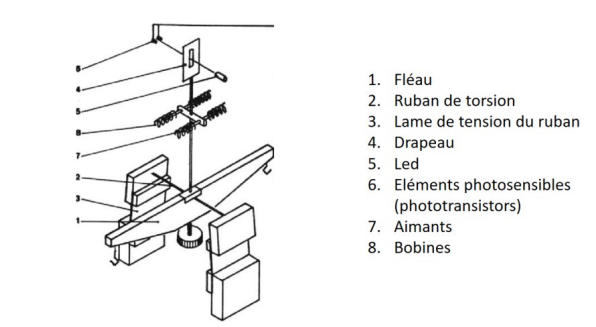
\includegraphics[scale=0.7]{C.png}
        \end{centering}
\end{figure}


\subsection{A}

\subsection{B}

\subsection{C}

\subsection{D}

\subsection{E}

\subsection{F}




\newpage

\section{Exercice 3 : Balance à fléau}
\begin{figure}[H]
	\begin{centering}
	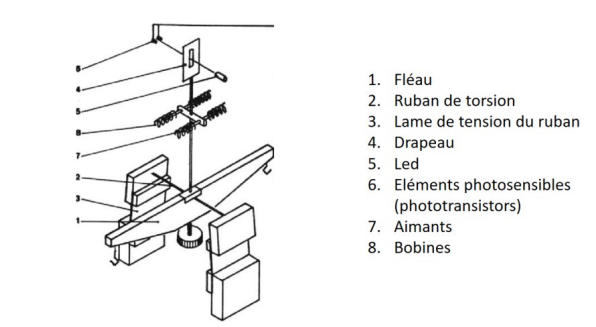
\includegraphics[scale=0.7]{C.png}
	\end{centering}
\end{figure}

\subsection{A}

\subsection{B}

\subsection{C}

\subsection{D}

\subsection{E}

\subsection{F}


\end{document}



